\documentclass[conference]{IEEEtran}
\IEEEoverridecommandlockouts

\usepackage{cite}
\usepackage{amsmath,amssymb}
\usepackage{graphicx}
\usepackage{booktabs}
\usepackage{array}
\usepackage{xcolor}
\usepackage[hyphens]{url}
\usepackage{tikz}
\usetikzlibrary{positioning,decorations.pathreplacing,calc}

% Markers for unfinished content. Search the source for \TODO, \VERIFY and \CITE.
\newcommand{\TODO}[1]{\textcolor{red}{\textbf{[TODO: #1]}}}
\newcommand{\VERIFY}[1]{\textcolor{orange}{\textbf{[VERIFY#1]}}}
\newcommand{\CITE}[1]{\textcolor{blue}{\textbf{[CITE#1]}}}
\newcommand{\shot}[2]{%
  \fbox{\parbox[c][#2][c]{0.94\linewidth}{\centering\footnotesize\textit{Headset capture placeholder:}\\ #1}}}

\begin{document}

\title{Templ-MR: Moving a Heritage Mixed Reality Application from HoloLens 2 to Meta Quest 3}

\author{
\IEEEauthorblockN{Aakash Choudary, Gautham Mohanraj, Hridesh MG, KK Surendran}
\IEEEauthorblockA{Department of Computer Science and Engineering \VERIFY{}\\
Amrita School of Computing, Amrita Vishwa Vidyapeetham\\
Amritapuri, Kollam, India\\
\VERIFY{: author emails}}
\and
\IEEEauthorblockN{Uma Gopalakrishnan}
\IEEEauthorblockA{Center for Wireless Networks \& Applications (WNA)\\
Amrita Vishwa Vidyapeetham\\
Amritapuri, India\\
umag@am.amrita.edu}
}

\maketitle

\begin{abstract}
KovilLens is a HoloLens 2 application that restores the ruined third shrine of Moovar Kovil, a 9th-century Chola temple complex, as a hologram that visitors can explore, listen to and watch collapse. HoloLens 2 is no longer manufactured, its toolkit is frozen at MRTK 2, and its cost limits deployment to a handful of headsets. We describe Templ-MR, a port of KovilLens to Meta Quest 3 using the Meta XR SDK and passthrough mixed reality. We compare the two platforms on cost, lifecycle, display, compute, input and co-location support, and map each KovilLens feature to its Quest 3 version, stating what was kept, redesigned and dropped. The port re-implements the destruction feature as a deterministic Voronoi pre-fracture of the 0.3-million-triangle model, with rubble that lands on the scanned room, is hidden by real objects through the Depth API, and can be picked up and thrown. We also present a colocated multi-user design built on Bluetooth discovery, a LAN host and room sharing. It is implemented end to end but does not yet align headsets reliably, so we report it as work in progress, with the failure we observed. Performance and user measurements are planned, and the protocol is given.
\end{abstract}

\begin{IEEEkeywords}
Cultural heritage, Mixed reality, HoloLens 2, Meta Quest 3, Video see-through, Porting, Colocated collaboration, Fracture simulation
\end{IEEEkeywords}

\section{Introduction}
Digital reconstruction lets visitors see heritage sites as they were before neglect and invasion damaged them~\cite{innocente2023,bec2021}. KovilLens~\cite{kovillens2025} applied this to Moovar Kovil in Kodumbalur, Tamil Nadu, a Chola-period complex~\cite{orr2007} where two of three near-identical shrines survive and the third stands only to its basement~\cite{kovillens2025}. On a Microsoft HoloLens 2, KovilLens shows the missing shrine as a hologram with a narrated tour, tooltips naming its parts, hand manipulation, and a simulated destruction. In a study with 23 participants, 87\% rated the storytelling mode as very effective and 96\% said they would recommend the application~\cite{kovillens2025}.

Two problems made us move the application. The first is the platform's future. Microsoft has ended HoloLens 2 production; the November 2024 release was the last feature update, and security fixes continue only until December 2027~\cite{hl2eol,hl2discontinued}. MRTK~2, on which KovilLens is built, stays at version~2 under Microsoft, while MRTK~3 moved to an independent organization~\cite{mrtk2repo,mrtk3}. Azure Spatial Anchors, the usual way to share coordinates between HoloLens devices, was retired on 20 November 2024~\cite{asaretire}. The second problem is scale. At US\$3,500 per headset~\cite{hl2price}, a site or classroom can afford one or two units, so the experience is used by one visitor at a time while others wait.

Meta Quest 3 is a consumer headset with colour passthrough, a depth sensor, hand tracking and a maintained SDK, priced at US\$499.99 for the 512\,GB model as of September 2024~\cite{q3price,q3compare}. Meta's SDK also offers Bluetooth colocation discovery and room sharing~\cite{metacolocation,metaspacesharing}, which make a shared, multi-visitor version of the temple feasible on headsets a group can afford. The cost is a change of display type: the real temple and the other visitors are seen through cameras rather than through glass.

This paper reports that move. Our contributions are:
\begin{enumerate}
\item A platform analysis of HoloLens 2 and Quest 3 for heritage mixed reality (MR), with every specification sourced, and an account of what the move gains and loses (Sections~\ref{sec:platform}, \ref{sec:discussion}).
\item A feature map from KovilLens to Templ-MR that names what was ported, redesigned, extended and not yet ported (Section~\ref{sec:design}).
\item A room-aware destruction system: a seeded Voronoi pre-fracture computed off the main thread, a staged collapse, and rubble that collides with the scanned room, is occluded by real objects and can be thrown (Section~\ref{sec:impl}).
\item A colocated multi-user design in which the deterministic fracture lets headsets share a collapse by streaming only piece poses. It is implemented but not yet working on two headsets; we report its state and the failures found so far (Section~\ref{sec:collab}).
\end{enumerate}

\section{Related Work}

\subsection{Heritage XR and KovilLens}
Immersive reconstructions have been used for destroyed sites, museum exhibits and tourism~\cite{innocente2023,bec2021,bozzelli2019}. Head-mounted MR in heritage has mostly meant HoloLens: Teruggi and Fassi tested HoloLens~2 spatial mapping inside Milan Cathedral~\cite{teruggi2022}, Hammady et al.\ studied visitor acceptance of an MR museum guide~\cite{hammady2020}, and Pedersen et al.\ argued for holographic displays in cultural heritage~\cite{pedersen2017}. KovilLens~\cite{kovillens2025} belongs to this line. Our group has also built a collaborative HoloLens~2 application for surgical planning~\cite{prabhakaran2024}. We found no published heritage MR application that was moved between headset families and evaluated before and after \CITE{: search further before submission}.

\subsection{Optical and video see-through}
Optical see-through (OST) displays such as HoloLens~2 show the real world directly and add light for virtual content; video see-through (VST) displays such as Quest~3 show camera images of the world with virtual content composited in. Rolland and Fuchs set out the trade-offs: VST controls occlusion and registration fully and can match latency between real and virtual, while OST keeps the real view at full resolution with no camera delay~\cite{rolland2000}. Itoh et al.\ survey the remaining OST problems, including limited field of view and the inability of additive displays to draw dark or opaque content~\cite{itoh2021}. For Quest~3 specifically, Vona et al.\ compared passthrough quality with Apple Vision Pro and Varjo XR-3 in reading and puzzle tasks; Quest~3 rated below Vision Pro on passthrough quality~\cite{vona2025}.

\subsection{Porting and colocated MR}
OpenXR gives a common runtime interface across headsets~\cite{openxr2019}, and both KovilLens and Templ-MR use Unity with OpenXR. Above that layer the toolkits differ: interaction, scene understanding and anchor sharing are vendor-specific, which is where most of the port's work lies. Colocated collaborative AR, where users share one physical space and see the same virtual objects in it, was argued for early by Billinghurst and Kato~\cite{billinghurst2002}. ViewR showed architectural-scale, multi-user MR on consumer VST headsets, with alignment, tracking-loss recovery and state synchronisation~\cite{schier2024}. Templ-MR targets the same setting at room scale, using vendor discovery and room sharing instead of a custom alignment step.

\section{Platform Analysis}\label{sec:platform}
Table~\ref{tab:platform} compares the two headsets. Specifications are vendor figures unless marked.

\begin{table}[t]
\caption{HoloLens 2 and Meta Quest 3 for Heritage MR}
\label{tab:platform}
\centering\footnotesize
\setlength{\tabcolsep}{3pt}
\begin{tabular}{@{}p{1.45cm}p{3.15cm}p{3.15cm}@{}}
\toprule
 & \textbf{HoloLens 2} & \textbf{Meta Quest 3} \\
\midrule
Price & US\$3,500 at launch~\cite{hl2price} & US\$499.99 (512\,GB), Sept.\ 2024~\cite{q3price} \VERIFY{: current price} \\
Lifecycle & Production ended; final feature release Nov.\ 2024; security fixes to Dec.\ 2027~\cite{hl2eol,hl2discontinued} & On sale; SDK v207 used here \\
Display & Waveguide OST, 2k 3:2 light engines~\cite{hl2hardware} & LCD VST, $2064{\times}2208$ per eye, 25\,PPD~\cite{q3compare} \\
Field of view & $52^\circ$ diagonal (press figure)~\cite{hl2fov} & $110^\circ$\,H, $96^\circ$\,V~\cite{q3compare} \\
Real-world view & Direct, through glass & Colour stereo passthrough, 4\,MP, 18\,PPD~\cite{q3compare} \\
Compute & Snapdragon 850, HPU 2.0, 4\,GB LPDDR4x~\cite{hl2hardware} & Snapdragon XR2 Gen~2, 8\,GB~\cite{q3compare} \\
Depth sensing & 1\,MP time-of-flight~\cite{hl2hardware} & Depth sensor, Depth API occlusion~\cite{q3compare,metadepth} \\
Input & Articulated hands, eye tracking, voice~\cite{hl2hardware} & Hands, Touch Plus controllers; no eye tracking~\cite{q3compare} \\
Weight & 566\,g~\cite{hl2hardware} & 515\,g~\cite{q3vrcompare} \VERIFY{: vendor figure} \\
Battery & 2--3\,h active~\cite{hl2hardware} & about 2\,h~\cite{q3compare} \\
Toolkit & MRTK~2 (frozen); MRTK~3 community-run~\cite{mrtk2repo,mrtk3} & Meta XR SDK: Core, Interaction SDK, MR Utility Kit \\
Co-location & Azure Spatial Anchors retired Nov.\ 2024~\cite{asaretire} & Bluetooth discovery, room sharing~\cite{metacolocation,metaspacesharing} \\
\bottomrule
\end{tabular}
\end{table}

\textit{Cost and lifecycle.} The price ratio is about seven to one. For a site that wants several visitors in the headset at once, this decides the matter more than any display figure. The lifecycle points the same way: a heritage installation is expected to run for years, and HoloLens~2 security support ends in December 2027~\cite{hl2eol}.

\textit{Display.} The field of view changes the experience most. On HoloLens~2 a life-size shrine is clipped to a window about $43^\circ{\times}29^\circ$~\cite{hl2fov}, so users step back or scale the temple down to see it whole. On Quest~3 the display spans $110^\circ$ horizontally, and VST lets the application decide what hides what: the Depth API supplies per-frame real-world depth for occlusion~\cite{metadepth}. In exchange, the real site, the guide and other visitors are seen at passthrough resolution, through cameras. For a reconstruction shown next to the real ruin this is a real loss, discussed in Section~\ref{sec:discussion}.

\textit{Compute and input.} Quest~3 has twice the memory. HoloLens~2 has eye tracking and voice input, neither of which KovilLens's code uses. Both support articulated hand tracking.

\textit{Co-location.} Sharing a coordinate frame is the precondition for a group experience. On HoloLens~2 the common cloud anchor service is retired~\cite{asaretire}; alternatives exist \CITE{: on-device or third-party HoloLens anchor sharing}, but none is part of the frozen MRTK~2 stack KovilLens uses. On Quest~3, colocation discovery advertises up to 1024 bytes of session data over Bluetooth~\cite{metacolocation}, and the MR Utility Kit can share a scanned room with a group so guests load the host's room~\cite{metaspacesharing}.

\section{System Design}\label{sec:design}
Templ-MR is a Unity 6 (6000.5.5f1) project on URP with Unity OpenXR 1.17.1, the Meta XR SDK 207.0.1 (Core, Interaction SDK, MR Utility Kit) and Netcode for GameObjects (NGO) 2.13.3. KovilLens used Unity 2022.3.19f1, the built-in render pipeline, MRTK 2.8.3 and Mixed Reality OpenXR 1.10.0. Both load the same temple model (about 299k triangles) and the same 88.9\,s narration. The project code grew from two scripts (429 lines) to fifteen (4,942 lines).

Fig.~\ref{fig:arch} shows the structure. Application modules sit on the Meta SDKs; multi-user wrappers sit on the modules and fall back to the single-user call when no session is running, so the single-user application is unchanged by networking.

\begin{figure}[t]
\centering
\resizebox{\columnwidth}{!}{% Templ-MR architecture. Layers bottom to top: device, SDKs, app modules, network wrappers.
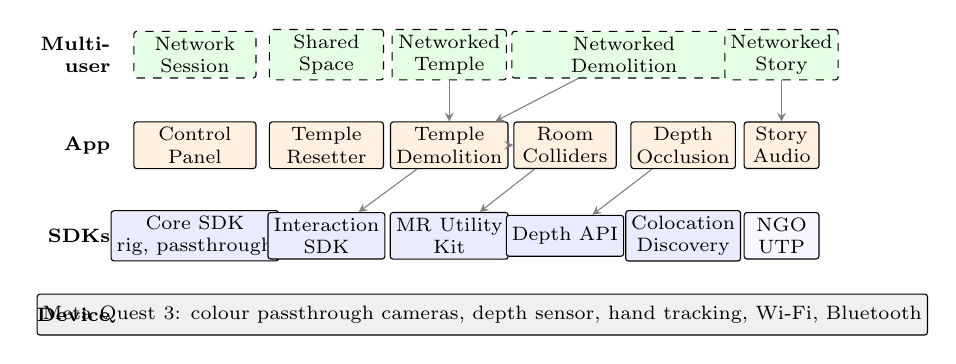
\begin{tikzpicture}[
  font=\scriptsize,
  layer/.style={draw, rounded corners=1pt, minimum height=5.2mm, inner sep=2pt, align=center},
  dev/.style={layer, fill=gray!12},
  sdk/.style={layer, fill=blue!8},
  app/.style={layer, fill=orange!12},
  net/.style={layer, fill=green!10, dashed},
  lbl/.style={font=\scriptsize\bfseries, anchor=east, align=right},
  >=stealth
]
% Device layer
\node[dev, minimum width=8.6cm] (dev) at (0.3,0)
  {Meta Quest 3: colour passthrough cameras, depth sensor, hand tracking, Wi-Fi, Bluetooth};
% SDK layer
\node[sdk, minimum width=1.55cm] (core) at (-3.35,1.0) {Core SDK\\rig, passthrough};
\node[sdk, minimum width=1.45cm] (isdk) at (-1.68,1.0) {Interaction\\SDK};
\node[sdk, minimum width=1.45cm] (mruk) at (-0.12,1.0) {MR Utility\\Kit};
\node[sdk, minimum width=1.30cm] (depth) at (1.35,1.0) {Depth API};
\node[sdk, minimum width=1.30cm] (coloc) at (2.85,1.0) {Colocation\\Discovery};
\node[sdk, minimum width=0.95cm, fill=blue!3] (ngo) at (4.1,1.0) {NGO\\UTP};
% App layer
\node[app, minimum width=1.55cm] (panel) at (-3.35,2.15) {Control\\Panel};
\node[app, minimum width=1.45cm] (reset) at (-1.68,2.15) {Temple\\Resetter};
\node[app, minimum width=1.45cm] (demo) at (-0.12,2.15) {Temple\\Demolition};
\node[app, minimum width=1.30cm] (room) at (1.35,2.15) {Room\\Colliders};
\node[app, minimum width=1.30cm] (occ) at (2.85,2.15) {Depth\\Occlusion};
\node[app, minimum width=0.95cm] (story) at (4.1,2.15) {Story\\Audio};
% Network layer
\node[net, minimum width=1.55cm] (sess) at (-3.35,3.3) {Network\\Session};
\node[net, minimum width=1.45cm] (space) at (-1.68,3.3) {Shared\\Space};
\node[net, minimum width=1.45cm] (ntemple) at (-0.12,3.3) {Networked\\Temple};
\node[net, minimum width=2.85cm] (ndemo) at (2.1,3.3) {Networked\\Demolition};
\node[net, minimum width=0.95cm] (nstory) at (4.1,3.3) {Networked\\Story};
% Layer labels
\node[lbl] at (-4.3,0) {Device};
\node[lbl] at (-4.3,1.0) {SDKs};
\node[lbl] at (-4.3,2.15) {App};
\node[lbl] at (-4.3,3.3) {Multi-\\user};
% Key dependencies between adjacent layers only, so no arrow crosses a box.
% Not drawn: NetworkSession uses Colocation Discovery and NGO; SharedSpace uses MRUK.
\draw[->, gray] (demo) -- (isdk);
\draw[->, gray] (room) -- (mruk);
\draw[->, gray] (occ) -- (depth);
\draw[->, gray] (ndemo) -- (demo);
\draw[->, gray] (ntemple) -- (demo);
\draw[->, gray] (nstory) -- (story);
\draw[->, gray] (demo) -- (room);
\end{tikzpicture}
}
\caption{Templ-MR architecture. Dashed boxes are the multi-user layer (work in progress). Network Session also uses Colocation Discovery and NGO; Shared Space uses the MR Utility Kit.}
\label{fig:arch}
\end{figure}

Table~\ref{tab:features} maps KovilLens features to Templ-MR. Two gaps are porting debt, not platform limits: the timed story sequence (light change, collapse at 25\,s, reset, and four tooltips naming adhisthana, bhitti, devakoshtas and vimana) and the mid-air ``Shatter'' mode. We removed far manipulation with hand rays on purpose and instead place the temple within arm's reach, so users interact only by poking and grabbing.

\begin{table}[t]
\caption{KovilLens Features in Templ-MR}
\label{tab:features}
\centering\footnotesize
\setlength{\tabcolsep}{3pt}
\begin{tabular}{@{}p{2.55cm}p{3.6cm}p{1.45cm}@{}}
\toprule
\textbf{KovilLens} & \textbf{Templ-MR} & \textbf{Status} \\
\midrule
Move, rotate, scale (MRTK) & ISDK grab, one or two hands, scale $0.2$--$5\times$ & Ported \\
Far (ray) manipulation \VERIFY{} & Removed; poke and grab only & Dropped \\
MRTK dashboard & Body-docked poke panel, built in code & Redesigned \\
`Anchor' & ``Set temple position'' & Ported \\
`Divine Restore' & ``Reset temple'' (also rebuilds) & Ported \\
Narrated tour & Play, pause, resume, progress bar & Ported \\
Timed animation, tooltips & -- & Not ported \\
``Collapse'' (explosion force on modelled parts) & Seeded Voronoi fracture, staged collapse & Rebuilt \\
``Shatter'' (pieces freeze mid-air) & -- & Not ported \\
Grab individual parts & Grab and throw pieces & Extended \\
Pieces fall to ground & Land on scanned floor and furniture & Extended \\
Occlusion by real objects & Depth API, floor-aware bias & Rebuilt \\
Single user & Colocated multi-user & In progress \\
\bottomrule
\end{tabular}
\end{table}

\section{Implementation}\label{sec:impl}

\subsection{Interaction and control panel}
At start the temple is placed in front of the user, its near side 0.5\,m from the eyes and turned to face them; that pose becomes ``home''. The temple uses the Interaction SDK's grabbable with a free transformer: one hand moves and rotates it, two hands also scale it, limited to 0.2--5 times its start size.

The MRTK dashboard became a panel that docks beside the body rather than the head, 0.24\,m to the side, 0.32\,m forward and 0.40\,m below the eyes, about the height of a lectern. Head-locked menus move whenever the user looks around, including when they turn to look at the menu. The panel instead follows a ``lazy'' body direction that changes only after the head stays turned more than $55^\circ$ for 0.8\,s, and never while the user looks within $35^\circ$ of the panel. A grab bar lets users move it; where it is dropped becomes its new place relative to the body. The panel holds the story controls, ``Reset temple'', ``Set temple position'', ``Demolish temple''/``Rebuild temple'', the session controls, and a developer popup for rescanning the room and showing the room colliders. Buttons that cannot act are greyed out, for example ``Reset'' while the temple lies in pieces. Every button fires on the press itself: during development, standard UI buttons, which fire on release, missed finger pokes that slid a few millimetres while pressed. The panel is built in code at start-up, with no prefabs or image assets. Fig.~\ref{fig:shots}(a) is a placeholder for a capture of it.

\subsection{Deterministic fracture}
KovilLens destroyed the temple by giving each modelled part a rigid body and applying one explosion force from a random point~\cite{kovillens2025}. The large shells of the model therefore fell as a few big pieces. Templ-MR cuts them itself, once, at start-up (Fig.~\ref{fig:fracture}):
\begin{enumerate}
\item Every mesh is transformed into temple space and classified. Meshes with at least 2,500 triangles, or larger than 12\% of the temple and with at least 200 triangles, are \emph{split}. Meshes smaller than 1.2\% of the temple are \emph{tiny} and ride on the nearest chunk. The rest (pillars, kalashas, statues) fall \emph{whole}.
\item 40 seed points are chosen from the split meshes' triangle centroids by best-candidate sampling (12 candidates per seed), which spreads the seeds evenly. The random generator is seeded with a constant, so every run and every device produces the same cut.
\item Each triangle is assigned to its nearest seed, a Voronoi partition of the surface. Each chunk's vertex and index buffers are rebuilt and pivoted on the chunk's centre. The model is dense enough that the jagged triangle borders read as broken stone.
\end{enumerate}
Steps 2--3 run on a worker thread so the headset keeps rendering; the button shows ``Preparing\ldots'' until they finish. Unlike volumetric fracture~\cite{muller2013}, this cut is surface-only and precomputed: chunks are hollow shells, so rubble materials are drawn double-sided. We chose it because it needs no solid model and costs nothing at demolition time. Its build time on the headset is \TODO{measure fracture build time on Quest 3}.

Each piece gets a box collider (at least 15\% of its largest extent thick), a rigid body with mass from its box volume at 2,500\,kg/m$^3$ (clamped to 0.02--50\,kg), continuous speculative collision so it does not tunnel through thin room surfaces, and a grabbable that throws on release. Box pairs that overlap in the intact temple are recorded. In the default ``explosive'' mode those overlaps push pieces apart and the rubble spreads across the room; otherwise collisions between them are ignored and the temple folds into a heap.

\begin{figure}[t]
\centering
\resizebox{\columnwidth}{!}{% Fracture and collapse pipeline in TempleDemolition.cs.
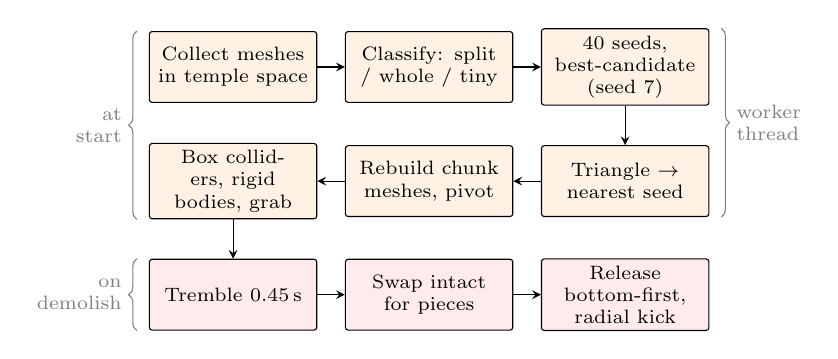
\begin{tikzpicture}[
  font=\scriptsize,
  stage/.style={draw, rounded corners=1pt, fill=orange!10, align=center, inner sep=2.5pt, text width=1.95cm, minimum height=9mm},
  run/.style={stage, fill=red!8},
  >=stealth, node distance=3.5mm
]
\node[stage] (a) {Collect meshes in temple space};
\node[stage, right=of a] (b) {Classify: split / whole / tiny};
\node[stage, right=of b] (c) {40 seeds, best-candidate (seed 7)};
\node[stage, below=5mm of c] (d) {Triangle $\rightarrow$ nearest seed};
\node[stage, left=of d] (e) {Rebuild chunk meshes, pivot};
\node[stage, left=of e] (f) {Box colliders, rigid bodies, grab};
\node[run, below=5mm of f] (g) {Tremble 0.45\,s};
\node[run, right=of g] (h) {Swap intact for pieces};
\node[run, right=of h] (i) {Release bottom-first, radial kick};
\draw[->] (a) -- (b); \draw[->] (b) -- (c); \draw[->] (c) -- (d);
\draw[->] (d) -- (e); \draw[->] (e) -- (f); \draw[->] (f) -- (g);
\draw[->] (g) -- (h); \draw[->] (h) -- (i);
\draw[decorate, decoration={brace, amplitude=3pt}, gray]
  ([xshift=1.5mm]c.north east) -- ([xshift=1.5mm]d.south east)
  node[midway, right=2pt, align=left, text=gray] {worker\\thread};
\draw[decorate, decoration={brace, amplitude=3pt, mirror}, gray]
  ([xshift=-1.5mm]a.north west) -- ([xshift=-1.5mm]f.south west)
  node[midway, left=2pt, align=right, text=gray] {at\\start};
\draw[decorate, decoration={brace, amplitude=3pt, mirror}, gray]
  ([xshift=-1.5mm]g.north west) -- ([xshift=-1.5mm]g.south west)
  node[midway, left=2pt, align=right, text=gray] {on\\demolish};
\end{tikzpicture}
}
\caption{Fracture at start-up and the collapse sequence on demolition.}
\label{fig:fracture}
\end{figure}

\subsection{Staged collapse}
On ``Demolish temple'' the temple trembles for 0.45\,s with an amplitude that ramps to 0.6\% of its height. It is then swapped for the pieces in place, and pieces are released from the bottom up over 0.3\,s according to their height. Each released piece gets a horizontal velocity that blends from an outward kick of 0.35 temple-heights per second at the base to an inward sag of 0.12 at the top, scaled by a random factor of 0.6--1.3, plus a random tumble. The base spreads while the top drops into it. Gravity is scaled by 0.75 for a heavier, slower fall. ``Rebuild temple'' restores the temple to where it stood before the collapse, not where its pieces landed.

\subsection{Room-aware rubble and occlusion}
At launch Templ-MR loads the headset's stored room scan through the MR Utility Kit and gives the floor, ceiling, walls, labelled furniture and the scanned room mesh invisible colliders, so rubble lands on the real floor and on tables and sofas (Fig.~\ref{fig:shots}(b)). Without a scan, rubble lands on an invisible plane at the temple's base. A coloured collider view in the developer popup lets us check the colliders against the room. We keep MRUK's world lock on: without it, the colliders were sometimes found shifted vertically after a demolition.

Occlusion uses the Depth API with soft edges~\cite{metadepth}. At start-up every opaque material is switched to a shader that applies Meta's occlusion test with two additions. First, virtual surfaces within 0.15\,m above the scanned floor need real surfaces to be much closer (a bias of 30\% of camera distance instead of 6\%) before they are hidden; otherwise depth noise lets the real floor swallow whatever rests on it. Second, hard, soft or no occlusion can be chosen per material. Rubble is never occluded, because soft occlusion left halos around small pieces. The user's real hands are removed from the depth used for occlusion, since tracked virtual hands are drawn.

\subsection{Narration}
The narration plays, pauses and resumes from where it stopped, with a progress bar and timer. KovilLens also locked manipulation and ran a timed sequence of light changes, a collapse and four tooltips during the tour~\cite{kovillens2025}; that sequence is not yet ported.

\subsection{Colocated multi-user (work in progress)}\label{sec:collab}
Fig.~\ref{fig:coloc} shows the session design.
(1)~The host starts an NGO host on UDP port 7777 on the local network, with no relay server, and advertises \texttt{"TempleMR/1 <ip> <port>"} over colocation discovery; the advertisement's UUID becomes the colocation group.
(2)~A guest pressing ``Join'' listens for 15\,s, parses the advertisement and connects; if nothing is found it falls back to a configured address.
(3)--(5)~The host shares its room with the group and sends each guest the group, room UUID and its floor-anchor pose. The guest loads the shared room, and the MR Utility Kit moves the guest's camera rig so the two floors coincide~\cite{metaspacesharing}. From then on, world coordinates should mean the same physical place on both headsets, and the guest's room colliders are the host's scan.
(6)--(7)~State is kept by the host:
\begin{itemize}
\item \emph{Temple.} The temple has an owner-authoritative network transform. Grabbing it asks the host for ownership, which is refused, and the grab cancelled, if another player holds it. Others cannot grab it meanwhile. The home pose lives on the host, so ``Set temple position'' and ``Reset temple'' from anyone apply for everyone.
\item \emph{Demolition.} Demolish and rebuild go through the host. Every headset plays the tremble and swaps in its own rubble; because the fracture is seeded, piece $i$ is the same chunk on every device, and only poses need to be sent. The host streams world-space poses of pieces that moved more than 1\,mm or $0.5^\circ$ at 15\,Hz over an unreliable channel, plus a full reliable snapshot every 2\,s and for late joiners. Each pose is 30 bytes (index, position, rotation), up to 32 per message, so the stream is bounded by about $15 \times 30N$ bytes per second for $N$ moving pieces, before transport overhead. Guests ease pieces toward the received poses. A guest holding a piece streams its pose to the host and, on release, sends the hand's measured velocity so the host continues the throw.
\item \emph{Narration.} The host stores whether the story is playing and the server time at which it started. Each headset plays the clip locally and seeks when it drifts more than 0.25\,s from that clock, so a late joiner starts at the current line.
\end{itemize}

\begin{figure}[t]
\centering
\resizebox{0.95\columnwidth}{!}{% Session set-up and alignment between a host and a guest headset (NetworkSession.cs, SharedSpace.cs).
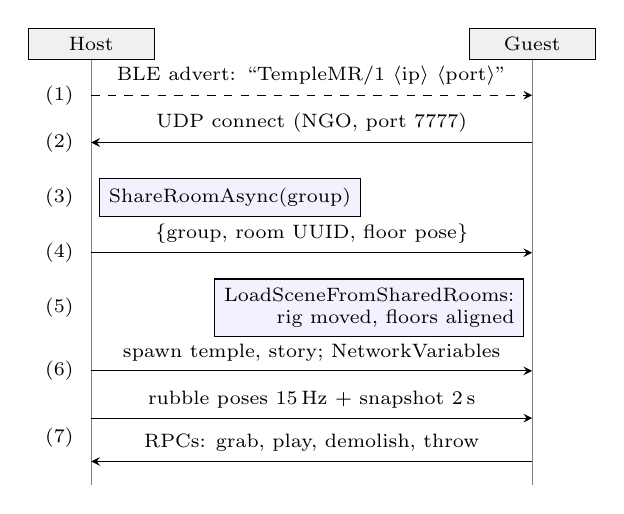
\begin{tikzpicture}[
  font=\scriptsize,
  msg/.style={->, >=stealth},
  note/.style={align=left, font=\scriptsize},
]
\def\top{0}
\def\bot{-5.6}
\node[draw, fill=gray!12, minimum width=1.6cm] (H) at (0,\top) {Host};
\node[draw, fill=gray!12, minimum width=1.6cm] (G) at (5.6,\top) {Guest};
\draw[gray] (H.south) -- (0,\bot);
\draw[gray] (G.south) -- (5.6,\bot);

\draw[msg, dashed] (0,-0.65) -- node[above, note] {BLE advert: ``TempleMR/1 $\langle$ip$\rangle$ $\langle$port$\rangle$''} (5.6,-0.65);
\node[note, anchor=east] at (-0.1,-0.65) {(1)};
\draw[msg] (5.6,-1.25) -- node[above, note] {UDP connect (NGO, port 7777)} (0,-1.25);
\node[note, anchor=east] at (-0.1,-1.25) {(2)};
\node[note, anchor=east, align=right] at (-0.1,-1.95) {(3)};
\node[note, anchor=west, draw, fill=blue!5] at (0.1,-1.95) {ShareRoomAsync(group)};
\draw[msg] (0,-2.65) -- node[above, note] {\{group, room UUID, floor pose\}} (5.6,-2.65);
\node[note, anchor=east] at (-0.1,-2.65) {(4)};
\node[note, anchor=east, draw, fill=blue!5, align=right] at (5.5,-3.35) {LoadSceneFromSharedRooms:\\rig moved, floors aligned};
\node[note, anchor=east] at (-0.1,-3.35) {(5)};
\draw[msg] (0,-4.15) -- node[above, note] {spawn temple, story; NetworkVariables} (5.6,-4.15);
\node[note, anchor=east] at (-0.1,-4.15) {(6)};
\draw[msg] (0,-4.75) -- node[above, note] {rubble poses 15\,Hz + snapshot 2\,s} (5.6,-4.75);
\draw[msg] (5.6,-5.3) -- node[above, note] {RPCs: grab, play, demolish, throw} (0,-5.3);
\node[note, anchor=east] at (-0.1,-5.0) {(7)};
\end{tikzpicture}
}
\caption{Session set-up, room alignment and state synchronisation.}
\label{fig:coloc}
\end{figure}

\textit{Status.} Session start and join were tested with the Unity Editor as host and one Quest~3. In the first two-headset test the guest found the host over Bluetooth, but its connection timed out without reaching the host; we suspect the phone hotspot used as the network. Once connected, the guest reported ``aligned'' but saw no temple, because NGO with scene management disabled destroys scene-placed network objects on a joining client~\cite{ngoinscene}; enabling scene management fixed this, and the guest's log then showed the temple at the host's coordinates. The guest still could not see it: the room alignment moved the guest's rig by about $(-0.26, -3.97, -0.41)$\,m, leaving the temple roughly 4\,m above the guest. Our leading hypothesis is that the host shared a stored room it was not standing in, since the code falls back to the first loaded room when the current room is unknown. Shared demolition, rubble streaming and synchronised narration have not yet been observed on two headsets.

\begin{figure}[t]
\centering
\shot{(a) Control panel docked at the user's side, expanded, with developer popup.}{2.3cm}\\[2pt]
\shot{(b) Rubble resting on the real floor and on a table after a collapse.}{2.3cm}
\caption{Templ-MR on Quest 3 (placeholders, see SCREENSHOTS\_NEEDED.md).}
\label{fig:shots}
\end{figure}

\section{Evaluation}\label{sec:eval}
No measurements of Templ-MR have been made yet. Table~\ref{tab:eval} lists what we will report and how; the full protocol is in the accompanying evaluation plan.

\begin{table}[t]
\caption{Planned Measurements}
\label{tab:eval}
\centering\footnotesize
\setlength{\tabcolsep}{3pt}
\begin{tabular}{@{}p{2.45cm}p{3.35cm}p{1.75cm}@{}}
\toprule
\textbf{Measure} & \textbf{Method} & \textbf{Result} \\
\midrule
Frame rate, frame time (idle, story, collapse, settled rubble) & OVR Metrics Tool, 60\,s per condition, 5 runs & \TODO{measure} \\
Fracture build time & Timestamp log around fracture at start-up & \TODO{measure} \\
Rubble piece count & Log piece count after fracture & \TODO{measure} \\
Collapse frame-time spike & Max frame time, 5\,s after Demolish & \TODO{measure} \\
Battery drain, thermals & Battery \% over a 20\,min session & \TODO{measure} \\
Alignment error (2 headsets) & Same physical marker touched on both & \TODO{measure} \\
Rubble stream bandwidth & Bytes sent per second, host & \TODO{measure} \\
Narration drift between headsets & Logged playback time vs server time & \TODO{measure} \\
Usability & SUS~\cite{brooke1996} & \TODO{measure} \\
Simulator sickness & SSQ~\cite{kennedy1993} & \TODO{measure} \\
KovilLens Likert items & Same 5 items as~\cite{kovillens2025} & \TODO{measure} \\
\bottomrule
\end{tabular}
\end{table}

\textit{Performance.} Each condition is recorded on a Quest~3 at the default refresh rate \VERIFY{: refresh rate used}, from a build without diagnostic logging.

\textit{Usability pilot.} A small pilot (\TODO{measure: N participants}) will complete the narrated tour, move and scale the temple, demolish it, pick up rubble, and rebuild, then fill in SUS, SSQ and the five Likert items KovilLens used~\cite{kovillens2025}, so the two builds can be compared item by item. The pilot will also ask, with the real ruin unavailable, how passthrough affects the sense of the temple standing in the room.

\textit{Feature parity.} Table~\ref{tab:features} is the parity check from the code. Each ``Ported'' row will also be confirmed on the headset \TODO{measure: on-device parity checklist}.

\section{Discussion and Limitations}\label{sec:discussion}
\textit{What we gained.} A headset at roughly one-seventh of the price, on a platform that is still sold and supported. A field of view that shows the life-size shrine without clipping. Depth-based occlusion and a labelled room model, which let rubble behave like objects in the room rather than holograms floating in front of it. And SDK support for discovery and room sharing, without which a shared visit would mean building our own anchor service.

\textit{What we lost.} The real world is now seen through cameras. At Moovar Kovil the point of the application is to stand next to the surviving shrines and see the missing one; on HoloLens~2 the surviving stone is seen directly, on Quest~3 it is seen at passthrough resolution, with the comfort costs Vona et al.\ measured~\cite{vona2025}. HoloLens~2 also has eye tracking and voice, which a future version of KovilLens might have used. Far interaction with hand rays was given up by choice. The KovilLens user study does not carry over; Templ-MR needs its own.

\textit{What is not yet ported.} The timed story sequence with tooltips and the ``Shatter'' mode. Both are application work, not platform limits, and both were among the features rated in the KovilLens study~\cite{kovillens2025}.

\textit{Limits of the new features.} The fracture is surface-only and fixed by its seed, so the temple always breaks the same way. Rubble is never occluded, so a piece behind a real chair is still drawn. Multi-user alignment does not work yet. Piece indices match across devices only if the fracture computes the same result on each; this holds for identical headsets but not between the Editor and a headset, and two players grabbing the same piece are not arbitrated. Templ-MR has not yet been taken to the site.

\section{Conclusion and Future Work}
We moved KovilLens from HoloLens 2 to Meta Quest 3 because the former is at the end of its life and too costly for group use. The move kept manipulation, reset, anchoring and narration, rebuilt destruction and occlusion around the room scan, and lost the direct view of the real site. Templ-MR's fracture is deterministic, which makes a shared collapse cheap to synchronise. Our next steps are, in order: fix multi-user room alignment and confirm the shared session on two or more headsets; port the timed story with tooltips and the ``Shatter'' mode; run the measurements and pilot in Section~\ref{sec:eval}; and test at Moovar Kovil itself, outdoors, next to the surviving shrines.

\section*{Acknowledgment}
We thank the authors of KovilLens for the application, model and narration this work builds on. \VERIFY{: funding and further acknowledgments, e.g. whether the KovilLens grant applies}

\bibliographystyle{IEEEtran}
\bibliography{refs}

\end{document}
